% Options for packages loaded elsewhere
\PassOptionsToPackage{unicode}{hyperref}
\PassOptionsToPackage{hyphens}{url}
\PassOptionsToPackage{dvipsnames,svgnames,x11names}{xcolor}
%
\documentclass[
]{article}

\usepackage{amsmath,amssymb}
\usepackage{iftex}
\ifPDFTeX
  \usepackage[T1]{fontenc}
  \usepackage[utf8]{inputenc}
  \usepackage{textcomp} % provide euro and other symbols
\else % if luatex or xetex
  \usepackage{unicode-math}
  \defaultfontfeatures{Scale=MatchLowercase}
  \defaultfontfeatures[\rmfamily]{Ligatures=TeX,Scale=1}
\fi
\usepackage{lmodern}
\ifPDFTeX\else  
    % xetex/luatex font selection
  \setmainfont[]{Latin Modern Roman}
  \setmathfont[]{Latin Modern Math}
\fi
% Use upquote if available, for straight quotes in verbatim environments
\IfFileExists{upquote.sty}{\usepackage{upquote}}{}
\IfFileExists{microtype.sty}{% use microtype if available
  \usepackage[]{microtype}
  \UseMicrotypeSet[protrusion]{basicmath} % disable protrusion for tt fonts
}{}
\makeatletter
\@ifundefined{KOMAClassName}{% if non-KOMA class
  \IfFileExists{parskip.sty}{%
    \usepackage{parskip}
  }{% else
    \setlength{\parindent}{0pt}
    \setlength{\parskip}{6pt plus 2pt minus 1pt}}
}{% if KOMA class
  \KOMAoptions{parskip=half}}
\makeatother
\usepackage{xcolor}
\setlength{\emergencystretch}{3em} % prevent overfull lines
\setcounter{secnumdepth}{5}
% Make \paragraph and \subparagraph free-standing
\ifx\paragraph\undefined\else
  \let\oldparagraph\paragraph
  \renewcommand{\paragraph}[1]{\oldparagraph{#1}\mbox{}}
\fi
\ifx\subparagraph\undefined\else
  \let\oldsubparagraph\subparagraph
  \renewcommand{\subparagraph}[1]{\oldsubparagraph{#1}\mbox{}}
\fi


\providecommand{\tightlist}{%
  \setlength{\itemsep}{0pt}\setlength{\parskip}{0pt}}\usepackage{longtable,booktabs,array}
\usepackage{calc} % for calculating minipage widths
% Correct order of tables after \paragraph or \subparagraph
\usepackage{etoolbox}
\makeatletter
\patchcmd\longtable{\par}{\if@noskipsec\mbox{}\fi\par}{}{}
\makeatother
% Allow footnotes in longtable head/foot
\IfFileExists{footnotehyper.sty}{\usepackage{footnotehyper}}{\usepackage{footnote}}
\makesavenoteenv{longtable}
\usepackage{graphicx}
\makeatletter
\def\maxwidth{\ifdim\Gin@nat@width>\linewidth\linewidth\else\Gin@nat@width\fi}
\def\maxheight{\ifdim\Gin@nat@height>\textheight\textheight\else\Gin@nat@height\fi}
\makeatother
% Scale images if necessary, so that they will not overflow the page
% margins by default, and it is still possible to overwrite the defaults
% using explicit options in \includegraphics[width, height, ...]{}
\setkeys{Gin}{width=\maxwidth,height=\maxheight,keepaspectratio}
% Set default figure placement to htbp
\makeatletter
\def\fps@figure{htbp}
\makeatother
\newlength{\cslhangindent}
\setlength{\cslhangindent}{1.5em}
\newlength{\csllabelwidth}
\setlength{\csllabelwidth}{3em}
\newlength{\cslentryspacingunit} % times entry-spacing
\setlength{\cslentryspacingunit}{\parskip}
\newenvironment{CSLReferences}[2] % #1 hanging-ident, #2 entry spacing
 {% don't indent paragraphs
  \setlength{\parindent}{0pt}
  % turn on hanging indent if param 1 is 1
  \ifodd #1
  \let\oldpar\par
  \def\par{\hangindent=\cslhangindent\oldpar}
  \fi
  % set entry spacing
  \setlength{\parskip}{#2\cslentryspacingunit}
 }%
 {}
\usepackage{calc}
\newcommand{\CSLBlock}[1]{#1\hfill\break}
\newcommand{\CSLLeftMargin}[1]{\parbox[t]{\csllabelwidth}{#1}}
\newcommand{\CSLRightInline}[1]{\parbox[t]{\linewidth - \csllabelwidth}{#1}\break}
\newcommand{\CSLIndent}[1]{\hspace{\cslhangindent}#1}

\usepackage{booktabs}
\usepackage{caption}
\usepackage{longtable}
\usepackage{array}
\usepackage{multirow}
\usepackage{wrapfig}
\usepackage{float}
\usepackage{colortbl}
\usepackage{pdflscape}
\usepackage{tabu}
\usepackage{threeparttable}
\usepackage{threeparttablex}
\usepackage[normalem]{ulem}
\usepackage{makecell}
\usepackage{xcolor}
\usepackage{tipa}
\usepackage{booktabs}
\usepackage{arxiv}
\usepackage{orcidlink}
\usepackage{amsmath}
\usepackage[T1]{fontenc}
\makeatletter
\makeatother
\makeatletter
\makeatother
\makeatletter
\@ifpackageloaded{caption}{}{\usepackage{caption}}
\AtBeginDocument{%
\ifdefined\contentsname
  \renewcommand*\contentsname{Table of contents}
\else
  \newcommand\contentsname{Table of contents}
\fi
\ifdefined\listfigurename
  \renewcommand*\listfigurename{List of Figures}
\else
  \newcommand\listfigurename{List of Figures}
\fi
\ifdefined\listtablename
  \renewcommand*\listtablename{List of Tables}
\else
  \newcommand\listtablename{List of Tables}
\fi
\ifdefined\figurename
  \renewcommand*\figurename{Figure}
\else
  \newcommand\figurename{Figure}
\fi
\ifdefined\tablename
  \renewcommand*\tablename{Table}
\else
  \newcommand\tablename{Table}
\fi
}
\@ifpackageloaded{float}{}{\usepackage{float}}
\floatstyle{ruled}
\@ifundefined{c@chapter}{\newfloat{codelisting}{h}{lop}}{\newfloat{codelisting}{h}{lop}[chapter]}
\floatname{codelisting}{Listing}
\newcommand*\listoflistings{\listof{codelisting}{List of Listings}}
\makeatother
\makeatletter
\@ifpackageloaded{caption}{}{\usepackage{caption}}
\@ifpackageloaded{subcaption}{}{\usepackage{subcaption}}
\makeatother
\makeatletter
\@ifpackageloaded{tcolorbox}{}{\usepackage[skins,breakable]{tcolorbox}}
\makeatother
\makeatletter
\@ifundefined{shadecolor}{\definecolor{shadecolor}{rgb}{.97, .97, .97}}
\makeatother
\makeatletter
\makeatother
\makeatletter
\makeatother
\ifLuaTeX
\usepackage[bidi=basic]{babel}
\else
\usepackage[bidi=default]{babel}
\fi
\babelprovide[main,import]{english}
% get rid of language-specific shorthands (see #6817):
\let\LanguageShortHands\languageshorthands
\def\languageshorthands#1{}
\ifLuaTeX
  \usepackage{selnolig}  % disable illegal ligatures
\fi
\IfFileExists{bookmark.sty}{\usepackage{bookmark}}{\usepackage{hyperref}}
\IfFileExists{xurl.sty}{\usepackage{xurl}}{} % add URL line breaks if available
\urlstyle{same} % disable monospaced font for URLs
\hypersetup{
  pdftitle={Cognate beginnings to bilingual lexical acquisition},
  pdfauthor={Gonzalo Garcia-Castro; Daniela S. Avila-Varela; Ignacio Castillejo; Nuria Sebastian-Galles},
  pdflang={en},
  pdfkeywords={cognate, word acquisition, vocabulary, bilingualism, item
response theory, bayesian},
  colorlinks=true,
  linkcolor={blue},
  filecolor={Maroon},
  citecolor={Blue},
  urlcolor={Blue},
  pdfcreator={LaTeX via pandoc}}

\usepackage{lineno}
\linenumbers
\usepackage{setspace}
\doublespacing
\newcommand{\runninghead}{A Preprint }
\renewcommand{\runninghead}{Cognate beginnings to bilingual lexical
acquistion }
\title{Cognate beginnings to bilingual lexical acquisition}
\author{
\textbf{Gonzalo Garcia-Castro}~\orcidlink{0000-0002-8553-4209}\\Center
for Brain and Cognition\\Universitat Pompeu Fabra\\Barcelona,
08005\\\href{mailto:gonzalo.garciadecastro@upf.edu}{gonzalo.garciadecastro@upf.edu}\\\\\\
\textbf{Daniela S. Avila-Varela}~\orcidlink{0000-0002-3518-8117}\\Center
for Brain and Cognition\\Universitat Pompeu Fabra\\Barcelona,
08005\\\href{mailto:avila.varela.daniela@gmail.com}{avila.varela.daniela@gmail.com}\\\\\\
\textbf{Ignacio
Castillejo}~\orcidlink{0000-0001-7445-0416}\\Departamento de
Psicología\\Universidad Autónoma de Madrid\\Madrid,
28049\\\href{mailto:jignaciocastillejo@gmail.com}{jignaciocastillejo@gmail.com}\\\\\\
\textbf{Nuria Sebastian-Galles}~\orcidlink{0000-0001-6938-2498}\\Center
for Brain and Cognition\\Universitat Pompeu Fabra\\Barcelona,
08005\\\href{mailto:nuria.sebastian@upf.edu}{nuria.sebastian@upf.edu}}
\date{}
\begin{document}
\maketitle
\begin{abstract}
Bilingual infants show equivalent developmental trajectories of lexical
acquisition compared to their monolingual peers. This is remarkable,
given the increased complexity of their linguistic input. Recent studies
suggested that bilingual vocabulary growth is boosted by the number of
cognates shared by the pair of languages being learned, and that this
facilitation effect is driven by a stronger parallel activation of
cognates during linguistic exposure, compared to non-cognates. The
mechanisms behind this facilitation are still unclear. In this study, we
capitalise on accumulator models of language acquisition to propose an
account of bilingual lexical acquisition in which parallel activation
increases the rate at which children accumulate learning instances for
words in both languages, even in fully monolingual situations. Under
this hypothesis, we predicted a stronger cognate facilitation for words
to which children were exposed less frequently (low-exposure words), as
they are co-activated by their translation more often than high-exposure
words do. We developed an extensive online vocabulary checklist, the
Barcelona Vocabulary questionnaire (BVQ) to collect vocabulary data from
366 Catalan-Spanish bilingual toddlers aged 12 to 32 months. We then
used Bayesian explanatory item response theory to model the acquisition
trajectories of 302 Catalan/Spanish translation equivalents. We found an
interaction between exposure and cognateness, which pointed to
cognateness facilitating the aquisition of low-exposure words, but not
of mean exposure or high-exposure words. Overall, our findings suggest
that cognateness plays a key role in bilingual lexical acquisition, and
provides evidence for a frequency-mediated facilitation effect driven by
parallel activation.
\end{abstract}
{\bfseries \emph Keywords}
\def\sep{\textbullet\ }
cognate \sep word
acquisition \sep vocabulary \sep bilingualism \sep item response
theory \sep 
bayesian

\ifdefined\Shaded\renewenvironment{Shaded}{\begin{tcolorbox}[interior hidden, borderline west={3pt}{0pt}{shadecolor}, breakable, enhanced, frame hidden, sharp corners, boxrule=0pt]}{\end{tcolorbox}}\fi

\hypertarget{introductionauthor-note}{%
\section[Introduction]{\texorpdfstring{Introduction\footnote{The authors
  declare no conflicts of interest with regard to the funding source of
  this study. This research was supported by grants from the Spanish
  Ministerio de Ciencia, Innovación y Universidades
  (PGC2018-101831-B-I00 and PRE2019-088165), and the Catalan Government
  {[}ICREA (Catalan Institution for Research and Advanced Studies)
  Academia 2019 award{]}. Gonzalo Garcia-Castro was supported by a
  fellowship of the Spanish Ministerio de Ciencia, Innovación y
  Universidades (FPI 2019). We are grateful to Chiara Santolin, Ege E.
  Özer, Alicia Franco-Martínez, Cristina Rodríguez-Prada, and the rest
  of the Speech Acquisition and Perception research group for their
  helpful feedback. We thank Xavier Mayoral, Silvia Blanch, and Cristina
  Cuadrado for their technical support, and Cristina Dominguez and Katia
  Pistrin for their efforts in recruiting infants. We also thank all
  families and infants who participated in the experiments.}}{Introduction}}\label{introductionauthor-note}}

The foundations of word learning are in place early in age. At six
months, infants start directing their gaze to some objects when hearing
their labels (\protect\hyperlink{ref-bergelson2012months}{Bergelson \&
Swingley, 2012}, \protect\hyperlink{ref-bergelson2015early}{2015};
\protect\hyperlink{ref-tincoff1999beginnings}{Tincoff \& Jusczyk,
1999}), and shortly after caregivers start reporting some words as
acquired by their infant in vocabulary checklists (e.g.,
\protect\hyperlink{ref-fenson2007macarthurbates}{Fenson et al., 2007};
\protect\hyperlink{ref-samuelson2021precision}{Samuelson, 2021}). Most
research on early word acquisition relies extensively on data from
monolingual children, and is oblivious to the fact that a substantial
proportion of the world population acquires more than one language from
early ages (\protect\hyperlink{ref-grosjean2021extent}{Grosjean, 2021}).
Previous work on bilingual vocabulary acquisition pointed to bilingual
toddlers knowing, on average, less words in each of their languages than
their monolinguals peers, and to both groups knowing a similar number of
words---if not more words---when the bilinguals' two languages are
pooled together. Hoff et al.
(\protect\hyperlink{ref-hoff2012dual}{2012}) found that English-Spanish
bilingual toddlers in South Florida (United States) knew less words in
English than monolinguals did, but both groups knew a similar total
amount of words when both English and Spanish vocabularies were counted
together. Other studies have provided converging evidence that
bilinguals know a similar or even larger number of words than
monolinguals when the two languages are aggregated
(\protect\hyperlink{ref-gonzalez-barrero2020bilingual}{Gonzalez-Barrero
et al., 2020}; \protect\hyperlink{ref-oller2002language}{Oller \&
Eilers, 2002}; \protect\hyperlink{ref-patterson2004comparing}{Patterson,
2004}; \protect\hyperlink{ref-patterson2004bilingual}{Patterson \&
Pearson, 2004}; \protect\hyperlink{ref-pearson1993lexical}{Pearson et
al., 1993}; \protect\hyperlink{ref-pearson1994patterns}{Pearson \&
Fernández, 1994}; \protect\hyperlink{ref-petitto2001bilingual}{Petitto
et al., 2001}; \protect\hyperlink{ref-smithson2014bilingualism}{Smithson
et al., 2014}). A more detailed analysis of the words in bilinguals'
lexicon show some interesting patterns.

One important observation of studies on bilinguals' early vocabulary
acquisition is that cognate words are easier to acquire than non-cognate
words. Cognate words are translation equivalents that are phonologically
similar (or share some type of form-similarity). For instance, the
Spanish translation equivalent of \emph{cat} is \emph{gato}, a cognate
word; the translation equivalent of \emph{dog} is \emph{perro}, a
non-cognate word. The differences in the percentages of cognate and
non-cognate words between two languages is related to historic reasons:
languages typologically close (like Dutch and English or Italian and
Spanish) share more cognates than languages typologically distant (like
English and Chinese, or Urdu and Spanish). The conclusion that cognate
words are easier to learn is based on two types of evidence: studies
investigating vocabulary sizes in children learning language pairs with
different percentages of cognates (that is, differing in their
typological distance) and studies comparing the number of cognate and
non-cognate words children know in a specific language pair.

Floccia et al. (\protect\hyperlink{ref-floccia2018introduction}{2018})
published an impressive study comparing vocabularies of children
learning several language pairs differing in their percentage of
cognates. The authors collected vocabulary data on word comprehension
and production from 372 24-month-old bilingual toddlers living in the
United Kingdom who were learning English and an additional language. The
additional language was one of 13 typologically diverse languages:
Bengali, Cantonese Chinese, Dutch, French, German, Greek, Hindi/Urdu,
Italian, Mandarin Chinese, Polish, Portuguese, Spanish and Welsh. The
authors calculated the average phonological overlap between the words in
each of these additional languages and their translation equivalents in
English, which was taken as a proxy of the degree of cognateness between
each pair of languages. Floccia and co-workers reported an increase in
vocabulary size in the additional language (i.e., not English)
associated with an increase in the average phonological similarity
between the translation equivalents of each language pair. For example,
English-Dutch bilinguals (languages with a high phonological overlap),
were able to produce more Dutch words than English-Mandarin bilinguals
(languages with a low phonological overlap) were able to produce in
Mandarin. Blom et al.
(\protect\hyperlink{ref-blom2020crosslanguage}{2020}), Bosma et al.
(\protect\hyperlink{ref-bosma2019longitudinal}{2019}), and Gampe et al.
(\protect\hyperlink{ref-gampe2021does}{2021}) reported similar results,
providing converging evidence of a facilitatory effect of language
distance on vocabulary size.

A second set of studies concluded that cognates are overrepresented in
bilinguals' early lexicon. Bosch \& Ramon-Casas
(\protect\hyperlink{ref-bosch2014first}{2014}) collected parental
reports of expressive vocabulary from 48 Catalan-Spanish bilinguals aged
18 months and found that cognates represented a larger proportion of
participant's vocabulary than non-cognates. Schelletter
(\protect\hyperlink{ref-schelletter2002effect}{2002}) provided
converging evidence from a longitudinal single-case study, in which an
English-German bilingual child produced cognates earlier than
non-cognates, on average. Mitchell et al.
(\protect\hyperlink{ref-mitchell2022cognates}{2022}) addressed this
issue in a larger sample longitudinal study. These authors collected
expressive vocabulary data of 47 16- to 30-month-old French-English
bilinguals living in Canada, in both languages. They created two lists
of translation equivalents: one made of 131 cognates, and one made of
406 non-cognates. The proportion of words that children were reportedly
able to produce was higher in the cognate lists than in the non-cognate
list across ages, even when both lists were matched by semantic category
(furniture, animals, food were similarity represented in both lists) and
age-of-acquisition norms (an index of word difficulty). Taken together,
the results of these two lines of research provide a strong support to
the hypothesis that phonological similarity (as reflected in
cognateness) plays a facilitation role in bilingual word acquisition.

Parallel activation of bilinguals' lexicons has been proposed as the
underlying mechanism for such facilitatory effect (e.g.,
\protect\hyperlink{ref-floccia2018introduction}{Floccia et al., 2018};
\protect\hyperlink{ref-mitchell2022cognates}{Mitchell et al., 2022}).
The parallel activation hypothesis stems from the language non-selective
account of lexical access, which suggests that bilinguals activate both
languages simultaneously during language processing, even in fully
monolingual contexts Evidence with adult bilinguals supporting the
language-non selective account of lexical access has been reported for
language comprehension and production, across the auditory and visual
(reading and signing) modalities
(\protect\hyperlink{ref-gimeno-martinez2021crosslinguistic}{Gimeno-Martínez
et al., 2021}; \protect\hyperlink{ref-vanhell2008sentence}{Hell \&
Groot, 2008}; \protect\hyperlink{ref-hoshino2008cognate}{Hoshino \&
Kroll, 2008}; \protect\hyperlink{ref-morford2011when}{Morford et al.,
2011}; \protect\hyperlink{ref-schwartz2007reading}{Schwartz et al.,
2007}; \protect\hyperlink{ref-spivey1999cross}{Spivey \& Marian, 1999};
see \protect\hyperlink{ref-kroll2017bilingual}{Kroll \& Ma, 2017} for
review). One of the clearest pieces of evidence of parallel activation
was provided by Costa et al.
(\protect\hyperlink{ref-costa2000cognate}{2000}). In this study, Spanish
monolinguals and Catalan-Spanish bilingual adults were asked to name
pictures of common objects in Spanish. In half of the trials, the object
labels were cognates in Spanish and Catalan (\emph{árbol}-\emph{arbre},
translations of \emph{tree}), whereas in the other half of the trial
labels were non-cognates (\emph{mesa}-\emph{taula}, translations of
\emph{table}), obviously, such distinction was only relevant for
bilinguals. Bilinguals named cognate pictures faster than non-cognate
pictures, even after adjusting for the lexical frequency of the items.
In contrast, Spanish monolinguals, who were unfamiliar with the Catalan
translations of the Spanish words they uttered, showed equivalent naming
times for the two types of stimuli. The authors interpreted the
difference between cognates and non-cognates in bilinguals as reflecting
the additional phonological activation that cognate words would receive
from their translation equivalents (due to language non-selective
activation of bilinguals' lexicons). These results showed that
bilinguals' Catalan phonology was activated during the production of
Spanish words, facilitating the naming of cognate pictures. Evidence of
parallel activation has been reported in bilingual toddlers and children
(\protect\hyperlink{ref-bosma2020cognate}{Bosma \& Nota, 2020};
\protect\hyperlink{ref-poarch2012crosslanguage}{Poarch \& Hell, 2012};
\protect\hyperlink{ref-poulin-dubois2013lexical}{Poulin-Dubois et al.,
2013}; \protect\hyperlink{ref-schroter2016orthographic}{Schröter \&
Schroeder, 2016}; \protect\hyperlink{ref-vonholzen2019impact}{Von Holzen
et al., 2019}; \protect\hyperlink{ref-vonholzen2012language}{Von Holzen
\& Mani, 2012}).

Although there is a consensus on the role of parallel activation in
bilinguals' lexical processing and acquisition, previous studies do not
address its influence on the learning trajectories of words. Results are
aggregated across words and provide no information about the specific
dynamics of how parallel activation influences word learning. This is
the goal of the present research.

We propose an account in which a learning instance for a word may also
represent a learning instance for its translation equivalent, to the
extent that such translation equivalent is co-activated\footnote{We use
  the term \emph{learning instance} in the fashion of accumulator models
  of language acquisition; as an exposure to a word-form that
  constitutes an opportunity for the child to accumulate information
  about the word. We do not make strong assumptions about whether a
  learning instance is a discrete or a continuous unit of accumulation
  of information. We rather consider that a learning instance of a word
  is so to the degree of the strength of activation of its phonological
  representation. This activation may be the result of the infant being
  exposed to the word-form, or the result of activation spreading
  through phonological or semantic links across lexicl representation,
  as in the case of parallel activation.}. The strength of this
co-activation is proportional to the phonological similarity between the
two translation equivalents; given that cognates share higher
phonological similarity than non-cognates, the former should be
co-activated more frequently than the latter. This should lead to a
faster accumulation of learning instances for cognates, compared to
non-cognates. Parallel activation would allow bilingual children to
accumulate learning instances for words in both languages even during
fully monolingual situations, but the impact of this mechanism would be
asymmetric across languages: words from the lower-exposure language
would receive additional activation through parallel activation more
often than words from the higher-exposure language. Therefore, the
acquisition of words from the lower-exposure language would benefit more
strongly from their cognate status than words from the higher-exposure
language.

Consider the example of the Catalan-Spanish cognate translation
equivalent /\textipa{"gat}-\textipa{"ga.to}/ {[}cat{]}, that are
phonologically very similar. When the child is exposed to
/\textipa{"gat}/, they will strongly co-activate /\textipa{"ga.to}/ in
parallel. Therefore, this exposure will count as a learning instance for
both co-activated forms. However, for the case of the non-cognate
translation equivalent /\textipa{"gos}/, the low phonological similarity
will result in a weak activation of /\textipa{"pe.ro}/ resulting in such
exposure counting as a learning instance for /\textipa{"gos}/ (which the
child was exposed to), but not for /\textipa{"pe.ro}/. While
/\textipa{"gat}-\textipa{"ga.to}/ will benefit from parallel activation,
/\textipa{"gos}-\textipa{"pe.ro}/ will not. If the child receives
linguistic input from one of the languages more often than from the
other, this effect might affect each form of the cognate translation
equivalent differently. For instance, if the child receives a larger
amount of Catalan input than Spanish input, they will encounter the
Catalan form /\textipa{"gat}/ more frequently than the Spanish form
/\textipa{"ga.to}/. Through parallel activation, /\textipa{"gat}/ will
activate /\textipa{"ga.to}/ more often than vice versa. Ultimately,
/\textipa{"ga.to}/ will benefit more strongly from its cognate status
than /\textipa{"gat}/, as it receives additional learning instances from
its translation equivalent more often than /\textipa{"gat}/.

To test these predictions, we collected vocabulary data on production
and comprehension from a large sample of bilingual Catalan-Spanish
children using an online vocabulary checklist designed for the present
study. We adopted a Bayesian explanatory item response theory approach
(IRT, see \protect\hyperlink{ref-kachergis2022standard}{Kachergis et
al., 2022}, for a similar approach) to model the probability of
acquisition of 604 Catalan and Spanish nouns included in the vocabulary
checklist. Words were considered as acquired if caregivers reported such
word to be understood (comprehension) or understood and said
(production) by their child. We estimated the impact of several
predictors of interest on the probability of acquisition, including
participants' age and rate of exposure to the word-form, and the cognate
status of the word-form. As described in the methods section, rate of
exposure was a composite measure taking into account participant'
language exposure and word's lexical frequency. We predicted an
interaction between cognate status and word exposure rate in which the
probability of comprehension is higher for low-exposure cognate words,
but not for high-exposure words cognate words.

\hypertarget{sec-methods}{%
\section{Methods}\label{sec-methods}}

All materials, data, and reproducible code can be found at the OSF
(\url{https://osf.io/hy984/}) and GitHub
(\url{https://github.com/gongcastro/cognate-beginnings}) repositories.
This study was conducted according to guidelines laid down in the
Declaration of Helsinki, and was approved by the Drug Research Ethical
Committee (CEIm) of the IMIM Parc de Salut Mar, reference 2020/9080/I.

\hypertarget{sec-questionnaire}{%
\subsection{Questionnaire}\label{sec-questionnaire}}

To collect vocabulary data from participants, we created an \emph{ad
hoc} questionnaire: the Barcelona Vocabulary Questionnaire (BVQ)
(\protect\hyperlink{ref-garcia-castro2023bvq}{Garcia-Castro et al.,
2023}). This questionnaire was inspired by the MacArthur-Bates
Communicative Development Inventory
(\protect\hyperlink{ref-fenson2007macarthurbates}{Fenson et al., 2007})
and its adaptations to other languages, and was implemented on-line
using the formr platform (\protect\hyperlink{ref-arslan2020formr}{Arslan
et al., 2020}). This questionnaire is structured in three blocks: (1) a
language exposure questionnaire, (2) a demographic survey, and (3) two
vocabulary checklists. Vocabulary checklists followed a similar
structure as the Oxford Communicative Developmental Inventory (OCDI)
(\protect\hyperlink{ref-hamilton2000infant}{Hamilton et al., 2000}) and
consisted in two lists of words: one in Catalan and one in Spanish. Both
lists included items from a diverse sample of 26 semantic/functional
categories. The Catalan checklist contained 793 items and the Spanish
checklist contained 797. Items in one language were translation
equivalents of the items in the other language (e.g., the same
participant responded to both \emph{gos} and \emph{perro}, Catalan and
Spanish for \emph{dog}), roughly following a one-to-one
mapping\footnote{Although for some of the included words in Catalan did
  not have a clear translation or had more than one possible translation
  in Spanish, and vice versa, therefore the unequal number of words
  included in the Catalan and Spanish lists} (see Table~\ref{tbl-items}
for a summary of the questionnaire items).

\hypertarget{tbl-items}{}
\begin{longtable}{l|rrrrc}
\caption{\label{tbl-items}Summary of the items included in the final analyses. }\tabularnewline

\toprule
\multicolumn{1}{l}{} & List A & List B & List C & List D & Examples \\ 
\midrule
\multicolumn{6}{l}{Semantic category} \\ 
\midrule
Household items & 31 & 26 & 30 & 25 & clock, video \\ 
Food and drink & 29 & 26 & 23 & 27 & sausage, yogurt \\ 
Animals & 26 & 23 & 19 & 25 & panther, tiger \\ 
Outside & 14 & 13 & 13 & 15 & farm, stone \\ 
Body parts & 14 & 12 & 11 & 11 & face, finger \\ 
Toys & 11 & 11 & 12 & 13 & piano, racket \\ 
Clothes & 12 & 12 & 10 & 10 & zipper, sandal \\ 
Vehicles & 9 & 10 & 11 & 10 & helicopter, tractor \\ 
Colours & 6 & 6 & 6 & 6 & red, green \\ 
People & 7 & 4 & 6 & 6 & police, babysitter \\ 
Furniture and rooms & 4 & 4 & 4 & 4 & corridor, terrace \\ 
Time & 2 & 2 & 2 & 2 & day, night \\ 
Adventures & 1 & 1 & 1 & 1 & witch \\ 
Parts of things & 1 & 1 & 1 & 1 & wheel \\ 
\midrule 
Total & 167 & 151 & 149 & 156 & — \\ 
\bottomrule
\end{longtable}

For each word included in the vocabulary checklists, we asked parents to
report whether their child was able to understand it, understand
\emph{and} say it, or did not understand or say it (checked out by
default). Given the large number of words in the vocabulary checklists,
we created four different subsets of the complete list of items. Each
subset contained a random but representative sub-sample of the items
from the complete list (see Table~\ref{tbl-items}). Semantic/functional
categories with less than 16 items---thus resulting in less than four
items after dividing it in four lists---were not divided in the short
version of the questionnaire: all of their items were included in the
four lists. Items that were part of the trial lists of some ongoing
experiments in the lab were also included in all versions. The resulting
reduced list contained between 343 and 349 Catalan words, and between
349 and 371 Spanish words. Participants were randomly allocated into one
of the four subsets.

To compute predictors of interest, we manually generated a broad
phonological transcription of every word included in the vocabulary
checklists in X-SAMPA format
(\protect\hyperlink{ref-wells1995computercoding}{Wells, 1995}). Catalan
word-forms were transcribed to Central Catalan phonology, and Spanish
word-forms were transcribed to Castilian Spanish phonology.

\hypertarget{sec-participants}{%
\subsection{Participants}\label{sec-participants}}

We collected 436 responses to the questionnaire from 366 distinct
children from the Metropolitan Area of Barcelona between the 30th of
March, 2020 and the 31th of October, 2022: 312 of those participants
participated once, 42 twice, 8 three times, and 4 four times. Recurrent
participants provided responses with a minimum of 25 days between
responses, and a maximum of 527, and were always allocated to the same
questionnaire list (A, B, C, or D). Participants were part of the
database of the Laboratori de Recerca en Infància (Universitat Pompeu
Fabra) and were contacted by e-mail or phone if their child was aged
between 12 and 32 months, and had not been reported to be exposed more
than 10\% of the time to a language other than Spanish or Catalan (see
Table~\ref{tbl-participants}) for a more detailed description of the
sample). In total, 70 participants (16.06\%) participants were reported
to be exposed to a third language other than Catalan and Spanish. All
families provided informed consent before participating. Upon consent,
families were sent a link to the questionnaire via e-mail, which they
filled from a computer, laptop, or mobile device. Filling the
questionnaire took 30 minutes approximately. After completion, families
were rewarded with a token of appreciation.

\hypertarget{tbl-participants}{}
\setlength{\LTpost}{0mm}
\begin{longtable}{rrrrrrr}
\caption{\label{tbl-participants}Participant sample size by age and degree of exposure to Catalan. }\tabularnewline

\toprule
 & \multicolumn{6}{c}{Age (months)} \\ 
\cmidrule(lr){2-7}
Catalan exposure\textsuperscript{\textit{1}} & [10,14] & (14,18] & (18,22] & (22,26] & (26,30] & (30,34] \\ 
\midrule
75-100\% & 18 & 23 & 36 & 38 & 20 & 7 \\ 
50-75\% & 8 & 13 & 30 & 41 & 18 & 1 \\ 
25-50\% & 10 & 17 & 45 & 29 & 17 & - \\ 
0-25\% & 7 & 11 & 21 & 17 & 8 & 1 \\ 
\bottomrule
\end{longtable}
\begin{minipage}{\linewidth}
\textsuperscript{\textit{1}}For participants exposed to Catalan and Spanish exclusively this proportion is complementary to the degree of exposue to Spanish. For participants exposed to a third languages this proportion is not complementary unless one adds the degree of exposed to the third language, which never exceeded 10\%.\\
\end{minipage}

We used the highest self-reported educational attainment of parents or
caregivers as a proxy of participants' socio-economic status (SES). This
information was provided by each parent or caregiver by selecting one of
six possible alternatives in line with the current educational system in
Spain: \emph{sense escolaritzar/sin escolarizar} {[}no education{]},
\emph{educació primària/educación primaria} {[}primary school{]},
\emph{educació secundària/educación secundaria} {[}secondary school{]},
\emph{batxillerat/bachillerato} {[}complementary studies/high school{]},
\emph{cicles formatius/ciclos formativos} {[}vocational training{]}, and
\emph{educació universitària/educación universitaria} {[}university
degree{]}. Most families reported university studies (356, 82\%),
followed by families were the highest educational attainment were
vocational studies (59, 14\%), secondary education (8, 2\%),
complementary studies (6, 1\%), primary education (1, \textless1\%), and
no formal education (2, \textless1\%).

\hypertarget{sec-analysis}{%
\subsection{Data analysis}\label{sec-analysis}}

We collected responses to 1,590 items. We restricted the analyses to
responses to nouns (628 items corresponding to other grammatical classes
were excluded, see \protect\hyperlink{ref-fourtassi2020growth}{Fourtassi
et al., 2020} for a similar approach). We then excluded items with
missing lexical frequency scores (\emph{n} = 269), items that included
more than one lemma (e.g., \emph{mono/mico} {[}monkey{]}, \emph{n} =
48), multi-word items or phrases (e.g., \emph{barrita de cereales}
{[}cereal bar{]}, \emph{n} = 9). Finally, we removed items without a
translation in the other language (\emph{n} = 32). This resulted in a
final list of 604 items, corresponding to words 302 Catalan words and
their 302 Spanish translations (302 translation equivalents). After
collecting participants' responses, the final dataset consisted of
138,078 observations, each corresponding to a single response of one
participant to one item. Each translation equivalent received a median
of 234 responses (\emph{Min} = 106, \emph{Max} = 872) from participants,
both languages pooled together.

We modelled the probability of participants answering each response
category (\emph{No} \textless{} \emph{Understands} \textless{}
\emph{Understands and Says}) using a Bayesian, multilevel, ordinal
regression model. This model allowed us to estimate both item and
participant word-acquisition trajectories, while estimating the effect
of our variables of interest: \emph{Age} (number of months elapsed
between participants' birth date and questionnaire completion),
\emph{Length} (number of phonemes in the X-SAMPA phonological
transcription of the word-form), \emph{Exposure} (a language
exposure-weighted lexical frequency), and \emph{Cognateness} (defined as
the phonological similarity between translation equivalentsFor each
translation equivalent). We added these variables as main effects,
together with the two-way and three-way interactions between \emph{Age},
\emph{Exposure}, and \emph{Cognateness}.

We developed the \emph{Exposure} predictor to account for the fact that
bilinguals' exposure to a given word-form is not only a function of the
word-forms lexical frequency, but also of the quantitative input they
receive from the language such word-form belongs to, we expressed
lexical frequencies as the product between both variables. First, we
extracted the child-directed lexical frequency of each word from the
CHILDES database
(\protect\hyperlink{ref-macwhinney2000childes}{MacWhinney, 2000};
\protect\hyperlink{ref-sanchez2019childesdb}{Sanchez et al., 2019}).
Using the corresponding lexical frequencies directly from Catalan and
Spanish was not possible due to the low number of Catalan participants
and tokens available in their corresponding CHILDES corpora, so they
were extracted from the English corpora instead. We then mapped the
lexical frequencies of the English words to their Catalan and Spanish
translations (see \protect\hyperlink{ref-fourtassi2020growth}{Fourtassi
et al., 2020} for a similar approach), and transformed them to Zipf
scores (\protect\hyperlink{ref-vanheuven2014subtlexuk}{Van Heuven et
al., 2014}; \protect\hyperlink{ref-zipf1949human}{Zipf, 1949}). We then
multiplied the resulting lexical frequencies by the reported degree of
exposure of the child to Catalan or Spanish. For instance, for a child
who is reportedly exposure to Catalan 80\% of the time, and to Spanish
20\% of the time, the expected exposure score to the Catalan word
\emph{cavall} {[}\emph{horse}{]}---with a lexical frequency of ---would
be , while that of its translation to Spanish \emph{caballo} would be .

We defined \emph{Cognateness} as the phonological similarity between
each word-form and its translation. For each translation equivalent, we
used the \texttt{stringdist}
(\protect\hyperlink{ref-vanderloo2014stringdist}{Loo, 2014}) R package
to calculate the Levenshtein distance between the Catalan and the
Spanish phonological transcriptions of the word-forms. The Levenshtein
distance measures the number of editions (insertions, deletions, or
substitutions) that one string of phonemes/characters must go through to
become identical to the other
(\protect\hyperlink{ref-levenshtein1966binary}{Levenshtein, 1966}). We
divided the Levnehstein distance of each translation equivalent by the
length of the longest word-form to correct for word length (longer
strings are likely to show a larger number of mismatches). Finally, we
subtracted the result from one so that it could be interpreted in terms
of phonological similarity, instead of phonological distance. This led
to a distance metric that ranged from zero to one, where zero indicates
that both word-forms are completely different (e.g., /'taw.l5-'me.sa/,
\emph{table}), and one indicates that the two word-forms are identical
(e.g., /'mar-'mar/, \emph{sea}) (see
\protect\hyperlink{ref-floccia2018introduction}{Floccia et al., 2018};
\protect\hyperlink{ref-fourtassi2020growth}{Fourtassi et al., 2020};
\protect\hyperlink{ref-heeringa2003norwegian}{Heeringa \& Gooskens,
2003}; \protect\hyperlink{ref-laing2022phonological}{Laing, 2022} for
similar approaches;
\protect\hyperlink{ref-schepens2012distributions}{Schepens et al.,
2012}).

Predictors were standardised before entering the model by subtracting
the mean of the predictor from each value and dividing the result by the
standard deviation of the predictor. Participant-level and item-level
random intercepts and slopes were included where appropriate, according
to the structure of the data
(\protect\hyperlink{ref-barr2013random}{Barr et al., 2013}). We
specified a weakly informative prior around the parameters of the model.
Equation~\ref{eq-linear} shows a detailed description of the model.

\begin{equation}\protect\hypertarget{eq-linear}{}{
\begin{aligned}
&\textbf{Response}~(k)~\textbf{to word}~i~ \textbf{by participant}~j \\
\text{Response}_{ij} &\sim \text{Cumulative logit}(\theta_{k_{ij}}) \\ 
&\text{where}~k \in \{\text{No} \rightarrow \text{Understands}, \text{Understands} \rightarrow \text{Understands and Says}\}\\
&\textbf{Distribution parameters} \\
\theta_{k_{ij}} &= (\beta_{0_{k}} + u_{0_{i_{k}}} + w_{0_{j_{k}}}) + (\beta_{1} + u_{1_{i}} + w_{1_{j}}) \cdot \text{Age}_{i} + \\
&(\beta_{2} + u_{2_{i}} + w_{2_{j}}) \cdot \text{Length}_{ij} + 
(\beta_{3} + u_{3_{i}} + w_{3_{j}}) \cdot \text{Exposure}_{ij} + & \\
& (\beta_{4} + u_{4_{i}}) \cdot \text{Cognateness}_{ij} + (\beta_{5} + u_{5_{i}} + w_{3_{j}}) \cdot (\text{Age}_{i} \times \text{Exposure}_{ij}) + & \\
& (\beta_{6} + u_{6_{i}}) \cdot (\text{Age}_{i} \times \text{Cognateness}_{ij}) + & \\
& (\beta_{7} + u_{7_{i}}) \cdot (\text{Exposure}_{ij} \times \text{Cognateness}_{ij}) & \\
& (\beta_{8} + u_{8_{i}}) \cdot (\text{Age}_{i} \times \text{Exposure}_{ij} \times \text{Cognateness}_{ij}) \\
&\text{where:}\\
& u_{1-8_{i}}~\text{: participant-level adjustments} \\
& w_{1-3_{j}}~\text{: TE-level adjustments} \\
&\textbf{Prior} \\
\beta_{0_{k}} &\sim \mathcal{N}(-0.25, 0.5); ~\beta_{1-5} \sim \mathcal{N}(0, 1) \\
\sigma_{u_{0-8}, w_{0-3}} &\sim \mathcal{N_{+}}(1, 0.25); ~\rho_{u_{0-8}, w_{0-3}} \sim \text{LKJcorr}(2) \\
&\text{where }~\rho_{u_{0-8}, w_{0-3}}~\text{are the correlations between group-level adjustments}\\
\end{aligned}
}\label{eq-linear}\end{equation}

We assessed the practical relevance of the estimated regression
coefficients of the model model following Kruschke \& Liddell
(\protect\hyperlink{ref-kruschke2018bayesian}{2018}). First, we
specified a region of practical equivalence (ROPE) from -2.5\% to
+2.5\%, in the probability scale. This region indicates the range of
values that we considered equivalent to zero. We then summarised the
posterior distribution of each regression coefficient with the 95\%
highest density interval (HDI). This interval contains the true value of
this coefficient with 95\% probability, given the data. Finally, we
calculated the proportion of posterior samples in the 95\% HDI that fell
into the ROPE, noted as \(p(\text{ROPE})\), which indicates the
probability that the true value of the regression coefficient falls into
the ROPE (and therefore should be considered equivalent to zero). For
example, a 80\% overlap between the HDI of a coefficient's posterior
distribution and the indicates that, given our data, there is a 80\%
probability that the true value of the coefficient falls within the
ROPE, and can therefore be considered equivalent to zero.

Data processing and visualisation was done in R
(\protect\hyperlink{ref-rcoreteam2013language}{R Core Team, 2013},
version 4.2.2) using the Tidyverse family of packages
(\protect\hyperlink{ref-wickham2019welcome}{Wickham et al., 2019}). We
implemented the model using \texttt{brms}
(\protect\hyperlink{ref-burkner2017brms}{Bürkner, 2017}), a R interface
to the Stan probabilistic language (2.32.1)
(\protect\hyperlink{ref-carpenter2017stan}{Carpenter et al., 2017}). We
ran four MCMC chains with 1,000 iterations each and an additional 1,000
warm-up iterations per chain. Model posterior draws and predictions were
handled using the \texttt{tidybayes}
(\protect\hyperlink{ref-kay2021tidybayes}{Kay, 2021}) and
\texttt{marginaleffects}
(\protect\hyperlink{ref-arel-bundock2022marginaleffects}{Arel-Bundock,
2022}) R packages.

\hypertarget{sec-results}{%
\section{Results}\label{sec-results}}

\renewcommand{\arraystretch}{1.25}

Model posterior showed adequate MCMC convergence diagnostics for all
parameters (\(\hat{R} \le 1.06\), \(0.022 \le N_{eff}/N < 1.1001\)) and
little evidence of multicollinearity. Table~\ref{tbl-coefs} shows the
summary of the posterior distribution of the fixed regression
coefficients, and their degree of overlap with the ROPE. For
interpretability, we report the estimated regression coefficients
transformed to the probability scale\footnote{The logit and probability
  scales relate non-linearly. This means that one logit difference is
  not necessarily translated to a unique value in the probability scale.
  For example, the probability of acquisition of a given word might
  increase in 5\% when age increases from 22 to 23 months, the
  probability of acquisition of the same word might only increase in
  0.2\% when age increases from 31 to 32 months. The linear growth of
  the probability of acquisition differs along the logistic curve, and
  therefore deciding the age point at which to report the estimates of
  the regression coefficients in the probability scale is not trivial.
  Following Gelman et al.
  (\protect\hyperlink{ref-gelman2020regression}{2020}), we report the
  maximum value of such coefficient, which corresponds to the linear
  growth (i.e.~derivative) of the logistic curve at the age at which
  most participants were acquiring a given word. This value can be
  approximated by dividing the coefficient in the logit scale by four:
  \(\hat{\beta_j}/4\), where \(\hat{\beta_j}\) is the estimated mean of
  the posterior distribution of coefficient \(j\).}. The resulting
values correspond to the maximum difference in probability of
acquisition (\emph{Comprehension} or \emph{Comprehension and
Production}) that corresponds to a one standard deviation change in each
predictor.

\hypertarget{tbl-coefs}{}
\begin{table}
\caption{\label{tbl-coefs}Posterior distribution of regression coefficients. }\tabularnewline

\centering
\begin{tabular}{lrlr}
\toprule
 & Median & 95\% HDI & $p(\text{ROPE})$\\
\midrule
\addlinespace[0.3em]
\multicolumn{4}{l}{\textbf{Intercepts (at 22 months)}}\\
\hspace{1em}Comprehension and Production & 0.4378 & {}[0.379, 0.496] & 0.0884\\
\hspace{1em}Comprehension & 0.9363 & {}[0.92, 0.949] & 0.0000\\
\addlinespace[0.3em]
\multicolumn{4}{l}{\textbf{Slopes (upper bound)}}\\
\hspace{1em}Age (+1 SD, 4.87, months) & 0.4049 & {}[0.357, 0.451] & 0.0000\\
\hspace{1em}Exposure (+1 SD, 1.81) & 0.2333 & {}[0.201, 0.268] & 0.0000\\
\hspace{1em}Cognateness (+1 SD, 0.26) & 0.0584 & {}[0.014, 0.104] & 0.0371\\
\hspace{1em}Length (+1 SD, 1.56 phonemes) & -0.0620 & {}[-0.086, -0.036] & 0.0000\\
\hspace{1em}Age $\times$ Exposure & 0.0714 & {}[0.039, 0.104] & 0.0000\\
\hspace{1em}Age $\times$ Cognateness & 0.0141 & {}[0, 0.026] & 0.9847\\
\hspace{1em}Exposure $\times$ Cognateness & -0.0569 & {}[-0.069, -0.046] & 0.0000\\
\hspace{1em}Age $\times$ Exposure $\times$ Cognateness & -0.0180 & {}[-0.027, -0.01] & 0.9747\\
\bottomrule
\end{tabular}
\end{table}

The main effect of \emph{Age} showed the strongest association with the
probability of acquisition (\(\beta\) = 0.405, 95\% HDI = {[}0.357,
0.451{]}), with all posterior samples falling out of the ROPE. A
one-month increment in age increased a maximum of 0.08 the probability
of acquisition. Similarly, the word exposure index (\emph{Exposure}) had
a strong effect on the probability of acquisition (\(\beta\) = 0.233,
95\% HDI = {[}0.201, 0.268{]}). All of the posterior samples of this
regression coefficient excluded the ROPE. The impact of this predictor
on the probability of acquisition was positive: for every standard
deviation increase in exposure, the participant was 0.129 more likely to
acquire it. Word-form length also showed a significant association with
probability of acquisition (\(\beta\) = -0.062, 95\% HDI = {[}-0.086,
-0.036{]}). For every phoneme in the word-form, participants were -0.04
less likely to know it. The 95\% HDI of the regression coefficient of
the \emph{Age} \(\times\) \emph{Exposure} interaction also excluded the
ROPE (\(\beta\) = 0.071, 95\% HDI = {[}0.039, 0.104{]}), showing that
the effect of the word exposure index differed across ages: older
children were more sensitive likely to acquire words with higher
exposure rate than younger children.

The posterior distribution of the main effect of cognateness excluded
the ROPE completely (\(\beta\) = 0.058, 95\% HDI = {[}0.014, 0.104{]}).
For every 10\% increment in cognateness, the acquisition of a word
increased in 0.006. The effect of \emph{Cognateness} interacted with
that of \emph{Exposure}: the 95\% HDI of the regression coefficient of
interaction excluded the ROPE entirely (\(\beta\) = -0.06, 95\% HDI =
{[}-0.069, -0.046{]}), suggesting that the effect of cognateness on a
word's probability of acquisition changed depending on participants'
exposure to word. Follow-up analyses on this interaction showed that
when exposure rate was low (e.g., -1 SD), cognateness increased the
probability of acquisition substantially. This effect was negligible
when for words with median or high exposure (+1 SD) (see
Figure~\ref{fig-marginal}).

\begin{figure}

{\centering 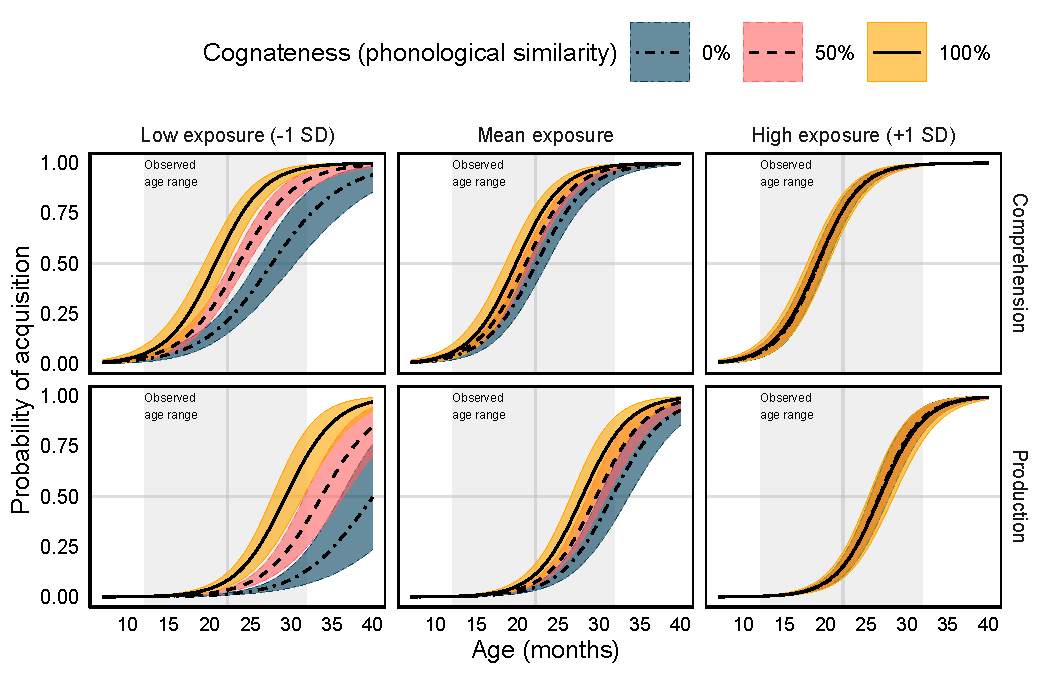
\includegraphics[width=1\textwidth,height=\textheight]{manuscript_files/figure-pdf/fig-marginal-1.pdf}

}

\caption{\label{fig-marginal}Posterior marginal effects. Lines
correspond to 100 posterior-predicted medians. Different colours
indicate different levels of cognateness (phonological similarity).
Predictions are presented separately for different degrees of word
exposure index: little exposure to the word, mean exposure, and high
exposure. Predictions for Comprehension are shown on top and predictions
for Comprehension and Production are shown on the bottom. In-sample
predictions lie inside the grey rectangles.}

\end{figure}

An additional analysis including lexical frequency and language exposure
as separate predictors (instead of the composite \emph{Exposure}
measure) showed equivalent results (see Appendix A). To rule out the
possibility that cognateness facilitation effect we found was due to
cognateness comprising more frequent syllables than non-cognates---and
therefore not because of their cognate status itself---, we compared the
syllabic frequency of cognates and non-cognates included in our
analyses. To calculate syllable frequency, we first extracted all
syllables embedded in the selected words. For each syllable, we summed
the lexical frequency of all the words in which such syllable appeared.
The resulting value provided an estimate of the number of times the
syllable appears in child-directed speech, embedded within different
words. Finally, for each word, we summed the frequency of its syllables,
as an estimate of the syllabic frequency of the word. We fit a Bayesian
model with \emph{Cognateness} as response variable, and the main effects
of syllable frequency and number of syllables (to control for the fact
words with more syllables are more likely to score higher in syllabic
frequency) as predictors. This model provided strong evidence for the
association between cognateness and syllabic frequency being equivalent
to zero (see Appendix B).

\hypertarget{sec-discussion}{%
\section{Discussion}\label{sec-discussion}}

This study investigated the impact of cognateness on the early bilingual
lexicon. We used Bayesian Item Response Theory to model the acquisition
trajectories of a large sample of Catalan and Spanish words, estimating
the effect of cognateness on the probability of acquisition. This model
corrected for participants' age, word-form length (number of phonemes),
and a novel measure of participants' exposure rate to each word.
Exposure rates were calculated as a language exposure-weighted lexical
frequency score in which each word-form's lexical frequency was
corrected by the degree to which the participant was exposed to each
language. Overall, we found that cognates (i.e., phonologically similar
translation equivalents) were acquired earlier than non-cognates. This
effect was mediated by exposure rate: low-exposure word-forms benefited
from their cognate status, whereas high-exposure word-forms did not.
Capitalising on accumulator models of language acquisition, we provide a
theoretical account of bilingual lexical acquisition. In this account,
parallel activation of the two languages plays a central role during the
consolidation of early representations in the bilingual lexicon, and in
which the dynamics of co-activation between translation equivalents
results in an earlier age-of-acquisition.

The present investigation is particularly relevant in the light of two
previous findings. First, Floccia et al.
(\protect\hyperlink{ref-floccia2018introduction}{2018}) reported that
bilingual toddlers learning two typologically close languages
(e.g.~shared many cognates, like., English-German) showed larger
vocabulary sizes than those learning typologically distant languages
(e.g.~shared fewer cognates, like English-Mandarin). Second, Mitchell et
al. (\protect\hyperlink{ref-mitchell2022cognates}{2022}) found an
earlier age-of-acquisition for cognates, compared to non-cognates. The
outcomes of both studies pointed to cognateness facilitating word
acquisition through parallel activation. But the underpinnings of such
effect were unclear: while parallel activation has been extensively
described in experimental studies, current paradigms of bilingual word
acquisition and word learning are, to a large extent, dissociated from
the mechanisms proposed by previous work on word processing. Accumulator
models of language acquisition may provide a convenient theoretical
framework to narrow this gap.

Accumulator models devise word acquisition as a continuous process in
which the child gathers information about words by accumulating learning
instances with such words. When the number of cumulative learning
instances for a word reaches some theoretical threshold, the child is
considered to have acquired such word. The rate at which a child
accumulates learning instances with a word is a function of child-level
properties (e.g., ability, amount of quantitative language exposure) and
word-level properties (e.g., lexical frequency)
(\protect\hyperlink{ref-hidaka2013computational}{Hidaka, 2013}). Through
statistical inference, formalised accumulator models provide meaningful
information about parameters of interest like the aforementioned
predictors (\protect\hyperlink{ref-kachergis2022standard}{Kachergis et
al., 2022}; \protect\hyperlink{ref-mollica2017how}{Mollica \&
Piantadosi, 2017}), and allow to generate quantitative predictions about
age-of-acquisition and vocabulary growth under competing theoretical
accounts (\protect\hyperlink{ref-hidaka2013computational}{Hidaka, 2013};
\protect\hyperlink{ref-mcmurray2007defusing}{McMurray, 2007}).
Capistalising on accumulator models, we extended this account to the
bilingual case, suggesting that the cognate facilitation effect on
bilingual word acquisition is the result of cognate words being
activated more strongly by their translation than non-cognates,
therefore accumulating learning instances at a faster rate. We
hypothesised that when a bilingual child is exposed to a word-form, they
activate not only its corresponding lexical representation, but also the
lexical representation of its translation. This cross-language
activation occurs at the phonological level, and the amount of
co-activation that spreads from the spoken word to its translation is
proportional to the amount of phonological similarity between both
word-forms. Cognates would receive more activation from their
translation than non-cognates, leading children to accumulate learning
instances with cognate words at a faster rate than with non-cognate
words. As a result, lexical representations of cognate words would
consolidate at earlier ages than those of non-cognate words.

These predictions address a critical subject in bilingualism research:
do bilingual infants accumulate learning experiences in both languages
independently, or does exposure to one language impact the acquisition
trajectory of the other language? In the context of lexical acquisition,
the former scenario predicts that every learning instance for a given
word-form contributes to the consolidation of the representation of such
word in the lexicon, while the consolidation of its translation remains
unaffected by such experience. In the latter scenario, a learning
instance to the same word-form would contribute not only to the
consolidation of the representation of such word, but also, to some
extent, to the consolidation of its translation. Our findings provide
strong support for an account of bilingual vocabulary growth in which
the experience and learning outcomes accumulated by the child in one
language impact those in the other language. Such a facilitatory
cross-language mechanism might be an important piece in the puzzle of
bilingual language acquisition. In particular, it may shed some light on
why bilingual infants do not show relevant delays in language
acquisition milestones compared to their monolingual peers, while
receiving a reduced quantity of speech input in each of their languages.
Our results provide some insights into this issue: infants benefited
more strongly from the cognateness facilitation effect when acquiring
words from the language of lower exposure than in the language of higher
exposure.

We suggest that this asymmetry is the result of children' unbalanced
exposure to their languages. A bilingual child's frequency of exposure
to a given word-form is mostly determined by two factors: the
word-form's lexical frequency and the child's amount of language
exposure to the language such word belongs to. A dual linguistic input
means lower exposure to each of the languages, unless one makes
the---arguably implausible---assumption that bilinguals are exposed on
average to twice the amount of linguistic input than monolinguals.
Because of this difference in exposure, words lower-exposure language
might receive activation from their translation in the higher-exposure
language more often than words from the higher-exposure language receive
activation from their translation in the lower-exposure language. As a
result, the cognateness facilitation effect should be stronger in words
from the lower-exposure language.

This mechanism might be extended to provide a plausible explanation for
the language similarity facilitation reported by Floccia et al.~The
authors observed a facilitation in the additional (non-English)
language: children learning two typologically close languages knew more
words in the additional language than those learning two typologically
more distant languages. In their sample, the additional language was
consistently also the lower-exposure language for most children, while
English was the higher-exposure language. Given that words in English
were more likely to be acquired first, higher phonological overlap for
words in the language of lower exposure (especially those of lower
lexical frequency) would facilitate vocabulary growth for languages
sharing more cognates with English.

It might be argued that our results reflect the fact that cognate
translation equivalents are represented in the initial bilingual lexicon
as the \emph{same} lexical entry. Because cognates correspond to similar
sounding word-forms in equivalent referential contexts (e.g., hearing
/\textipa{"gat}\}/ and /\textipa{"ga.to}\}/ in the presence of a cat),
it is possible that infants classify both are as acceptable variations
of the same word, therefore treating them as a single lexical item. This
would lead to a faster increase in cumulative learning instances, and to
earlier ages of acquisition for cognate translation equivalents (for
which listening to each word-form contributes to the acquisition of its
shared representation), compared to non-cognates (for which listening to
each word-form contributes to the acquisition of a separate
representation). This mechanism could potentially explain the earlier
age-of-acquisition effect of cognates found in the present study,
without the need of parallel activation playing any relevant role.
Mitchell et al. (\protect\hyperlink{ref-mitchell2022cognates}{2022})
discuss this possibility as a possible explanation of the cognate
facilitation effect, in which bilinguals only need to map one word-form
to the referent in the case of cognates, while mapping two distinct
word-forms in the case of non-cognates. However, previous work on
mispronunciation perception and learning of minimal pair words points in
a different direction. Bilingual toddlers show monolingual-level
sensitivity to slight phonetic changes in a word-form, according to
their performance in word recognition tasks
(\protect\hyperlink{ref-bailey2002phonological}{Bailey \& Plunkett,
2002}; \protect\hyperlink{ref-mani2011does}{Mani \& Plunkett, 2011};
\protect\hyperlink{ref-ramon-casas2009vowel}{Ramon-Casas et al., 2009},
\protect\hyperlink{ref-ramon-casas2017minimalpair}{2017};
\protect\hyperlink{ref-ramon-casas2010are}{Ramon-Casas \& Bosch, 2010};
\protect\hyperlink{ref-swingley200511montholds}{Swingley, 2005};
\protect\hyperlink{ref-swingley2000spoken}{Swingley \& Aslin, 2000};
\protect\hyperlink{ref-tamasi2017pupillometry}{Tamási et al., 2017};
\protect\hyperlink{ref-wewalaarachchi2017vowels}{Wewalaarachchi et al.,
2017}). The ability to differentiate between similar-sounding word-forms
is also reflected in word learning, as bilinguals seem to be able to map
minimal pairs to distinct referents
(\protect\hyperlink{ref-havy2016phonetic}{Havy et al., 2016};
\protect\hyperlink{ref-mattock2010first}{Mattock et al., 2010};
\protect\hyperlink{ref-ramon-casas2017minimalpair}{Ramon-Casas et al.,
2017}). Overall, it seems that bilinguals consider small differences in
the phonological forms of words as relevant at the lexical level. We
argue that this shows evidence that bilingual toddlers likely form
distinct lexical representations for even near-identical cognates.

Our study shares similar methodological limitations with previous work
using vocabulary reports provided by caregivers. Such reports can be
subject to measurement error induced by caregivers who may sometimes
overestimate or underestimate participants' true probability of
acquisition of words (e.g.,
\protect\hyperlink{ref-houston-price2007discrepancy}{Houston-Price et
al., 2007}). In the case of bilingual research additional biases may be
in place. Although in the present study caregivers were explicitly
instructed \emph{not} to rely on their responses to Catalan words when
responding to Spanish (and vice versa), it is possible that some
caregivers assumed---at least to some extent---that because the child
knew a word in one language, the child should also know the word in the
other language. This bias would especially affect similar-sounding
words, i.e., cognates. Production estimates may be more prompt to such
biases, in part because of the slower pace at which infants'
articulatory abilities develop, compared to their word recognition
abilities (\protect\hyperlink{ref-hustad2020development}{Hustad et al.,
2020}, \protect\hyperlink{ref-hustad2021speech}{2021}). This gap between
comprehension and production is even larger in the less dominant
language of bilingual children
(\protect\hyperlink{ref-giguere2022bilingual}{Giguere \& Hoff, 2022}).
For this reason, caregivers may be more uncertain about what words can
be counted as \emph{acquired} in this modality. Despite such potential
biases, vocabulary checklist filled by parents show strong evidence of
concurrent validity with other estimates of vocabulary size or lexical
processing (\protect\hyperlink{ref-feldman2005concurrent}{Feldman et
al., 2005}; \protect\hyperlink{ref-gillen2021tapping}{Gillen et al.,
2021}; \protect\hyperlink{ref-killing2008move}{Killing \& Bishop, 2008};
but see
\protect\hyperlink{ref-houston-price2007discrepancy}{Houston-Price et
al., 2007}).

The present study contributes with a specific data point to the complex
landscape of bilingualism research. Bilinguals are a remarkably
heterogeneous population difficult to be satisfactorily characterised in
a comprehensive way
(\protect\hyperlink{ref-sebastian-galles2020bilingual}{Sebastian-Galles
\& Santolin, 2020}). Bilinguals differ across multiple dimensions. Such
differences span from exclusively linguistic factors such as the amount
of overlap between the phonemic inventories of the two languages being
learned (e.g., low, like the case of English and Mandarin, or high like
the case of Spanish and Greek), to higher-level factors like the
socio-linguistic situation in which the two languages co-exist (e.g., in
some regions both languages are co-official and used in similar
contexts, while in others, one of the languages hardly has any societal
presence, i.e., heritage languages). This diversity of situations in
which bilingual toddlers acquire language calls for special
consideration of the generalisability of results in bilingualism
research. Our sample, although homogeneous (e.g., similar parental
educational level across), represents a particular bilingual
sociolinguistic environment: the languages involved in the present
investigation, Catalan and Spanish, co-exist in Catalonia as official
languages, both languages are used in fairly similar contexts, and both
languages are known by the majority of the population. In 2018, more
than 81.2\% of a representative sample of 8,780 adults aged 15 years or
older living in Catalonia reported being able to speak Catalan, and more
than 99.5\% of the same population reported being able to speak Spanish
(\protect\hyperlink{ref-2018els}{\emph{Els Usos Lingüístics de La
Població de Catalunya}, 2018}). In addition, Catalan and Spanish are
Romance languages and share a considerable amount of cognates. Extending
our analyses to other bilingual populations learning typologically more
distant languages, and whose languages tend to be used in more distinct
contexts (e.g., heritage languages) should be a natural future step for
the present investigation.

To conclude, our study provides novel insights about word acquisition in
bilingual contexts, and how the presence of cognates in the children's
linguistic input impacts the early formation of the lexicon. We found
that during the acquisition of low frequency words, bilingual children
seem to benefit more strongly from the word's phonological similarity
with its translation in the other language. Capitalising on accumulator
models of language acquisition we put forward a theoretical account of
bilingual word learning, in which cognateness interacts with lexical
frequency and language exposure to boost the acquisition of translation
equivalents.

\hypertarget{refs}{}
\begin{CSLReferences}{1}{0}
\leavevmode\vadjust pre{\hypertarget{ref-arel-bundock2022marginaleffects}{}}%
Arel-Bundock, V. (2022). \emph{Marginaleffects: Marginal effects,
marginal means, predictions, and contrasts}.
\url{https://CRAN.R-project.org/package=marginaleffects}

\leavevmode\vadjust pre{\hypertarget{ref-arslan2020formr}{}}%
Arslan, R. C., Walther, M. P., \& Tata, C. S. (2020). Formr: A study
framework allowing for automated feedback generation and complex
longitudinal experience-sampling studies using r. \emph{Behavior
Research Methods}, \emph{52}(1), 376--387.
\url{https://doi.org/10.3758/s13428-019-01236-y}

\leavevmode\vadjust pre{\hypertarget{ref-bailey2002phonological}{}}%
Bailey, T. M., \& Plunkett, K. (2002). Phonological specificity in early
words. \emph{Cognitive Development}, \emph{17}(2), 1265--1282.
\url{https://doi.org/10.1016/S0885-2014(02)00116-8}

\leavevmode\vadjust pre{\hypertarget{ref-barr2013random}{}}%
Barr, D. J., Levy, R., Scheepers, C., \& Tily, H. J. (2013). Random
effects structure for confirmatory hypothesis testing: Keep it maximal.
\emph{Journal of Memory and Language}, \emph{68}(3), 255--278.

\leavevmode\vadjust pre{\hypertarget{ref-bergelson2012months}{}}%
Bergelson, E., \& Swingley, D. (2012). At 6--9 months, human infants
know the meanings of many common nouns. \emph{Proceedings of the
National Academy of Sciences}, \emph{109}(9), 3253--3258.
\url{https://doi.org/10.1073/pnas.1113380109}

\leavevmode\vadjust pre{\hypertarget{ref-bergelson2015early}{}}%
Bergelson, E., \& Swingley, D. (2015). Early word comprehension in
infants: Replication and extension. \emph{Language Learning and
Development}, \emph{11}(4), 369--380.
\url{https://doi.org/10.1080/15475441.2014.979387}

\leavevmode\vadjust pre{\hypertarget{ref-blom2020crosslanguage}{}}%
Blom, E., Boerma, T., Bosma, E., Cornips, L., Heuij, K. van den, \&
Timmermeister, M. (2020). Cross-language distance influences receptive
vocabulary outcomes of bilingual children. \emph{First Language},
\emph{40}(2), 151--171. \url{https://doi.org/10.1177/0142723719892794}

\leavevmode\vadjust pre{\hypertarget{ref-bosch2014first}{}}%
Bosch, L., \& Ramon-Casas, M. (2014). First translation equivalents in
bilingual toddlers' expressive vocabulary: Does form similarity matter?
\emph{International Journal of Behavioral Development}, \emph{38}(4),
317--322. \url{https://doi.org/10.1177/0165025414532559}

\leavevmode\vadjust pre{\hypertarget{ref-bosma2019longitudinal}{}}%
Bosma, E., Blom, E., Hoekstra, E., \& Versloot, A. (2019). A
longitudinal study on the gradual cognate facilitation effect in
bilingual children's frisian receptive vocabulary. \emph{International
Journal of Bilingual Education and Bilingualism}, \emph{22}(4),
371--385. \url{https://doi.org/10.1080/13670050.2016.1254152}

\leavevmode\vadjust pre{\hypertarget{ref-bosma2020cognate}{}}%
Bosma, E., \& Nota, N. (2020). Cognate facilitation in frisian--dutch
bilingual children's sentence reading: An eye-tracking study.
\emph{Journal of Experimental Child Psychology}, \emph{189}, 104699.

\leavevmode\vadjust pre{\hypertarget{ref-burkner2017brms}{}}%
Bürkner, P.-C. (2017). Brms: An r package for bayesian multilevel models
using stan. \emph{Journal of Statistical Software}, \emph{80}, 1--28.
\url{https://doi.org/10.18637/jss.v080.i01}

\leavevmode\vadjust pre{\hypertarget{ref-carpenter2017stan}{}}%
Carpenter, B., Gelman, A., Hoffman, M. D., Lee, D., Goodrich, B.,
Betancourt, M., Brubaker, M., Guo, J., Li, P., \& Riddell, A. (2017).
Stan : A probabilistic programming language. \emph{Journal of
Statistical Software}, \emph{76}(1).
\url{https://doi.org/10.18637/jss.v076.i01}

\leavevmode\vadjust pre{\hypertarget{ref-costa2000cognate}{}}%
Costa, A., Caramazza, A., \& Sebastian-Galles, N. (2000). The cognate
facilitation effect: Implications for models of lexical access.
\emph{Journal of Experimental Psychology: Learning, Memory, and
Cognition}, \emph{26}, 1283--1296.
\url{https://doi.org/10.1037/0278-7393.26.5.1283}

\leavevmode\vadjust pre{\hypertarget{ref-2018els}{}}%
\emph{Els usos lingüístics de la població de catalunya}. (2018).
Generalitat de Catalunya.
\url{https://llengua.gencat.cat/web/.content/documents/dadesestudis/altres/arxius/dossier-eulp-2018.pdf}

\leavevmode\vadjust pre{\hypertarget{ref-feldman2005concurrent}{}}%
Feldman, H. M., Dale, P. S., Campbell, T. F., Colborn, D. K.,
Kurs-Lasky, M., Rockette, H. E., \& Paradise, J. L. (2005). Concurrent
and predictive validity of parent reports of child language at ages 2
and 3 years. \emph{Child Development}, \emph{76}(4), 856--868.
\url{https://doi.org/10.1111/j.1467-8624.2005.00882.x}

\leavevmode\vadjust pre{\hypertarget{ref-fenson2007macarthurbates}{}}%
Fenson, L. et al. (2007). \emph{{MacArthur}-bates communicative
development inventories}. Paul H. Brookes Publishing Company Baltimore,
{MD}.

\leavevmode\vadjust pre{\hypertarget{ref-floccia2018introduction}{}}%
Floccia, C., Sambrook, T. D., Delle Luche, C., Kwok, R., Goslin, J.,
White, L., Cattani, A., Sullivan, E., Abbot‐Smith, K., Krott, A., Mills,
D., Rowland, C., Gervain, J., \& Plunkett, K. (2018). I: introduction.
\emph{Monographs of the Society for Research in Child Development},
\emph{83}(1), 7--29. \url{https://doi.org/10.1111/mono.12348}

\leavevmode\vadjust pre{\hypertarget{ref-fourtassi2020growth}{}}%
Fourtassi, A., Bian, Y., \& Frank, M. C. (2020). The growth of
children's semantic and phonological networks: Insight from 10
languages. \emph{Cognitive Science}, \emph{44}(7), e12847.
\url{https://doi.org/10.1111/cogs.12847}

\leavevmode\vadjust pre{\hypertarget{ref-gampe2021does}{}}%
Gampe, A., Quick, A. E., \& Daum, M. M. (2021). Does linguistic
similarity affect early simultaneous bilingual language acquisition?
\emph{Journal of Language Contact}, \emph{13}(3), 482--500.

\leavevmode\vadjust pre{\hypertarget{ref-garcia-castro2023bvq}{}}%
Garcia-Castro, G., Ávila-Varela, D. S., \& Sebastian-Galles, N. (2023).
\emph{Bvq: Barcelona vocabulary questionnaire database and helper
functions}. \url{https://gongcastro.github.io/bvq}

\leavevmode\vadjust pre{\hypertarget{ref-gelman2020regression}{}}%
Gelman, A., Hill, J., \& Vehtari, A. (2020). \emph{Regression and other
stories}. Cambridge University Press.

\leavevmode\vadjust pre{\hypertarget{ref-giguere2022bilingual}{}}%
Giguere, D., \& Hoff, E. (2022). Bilingual development in the receptive
and expressive domains: They differ. \emph{International Journal of
Bilingual Education and Bilingualism}, \emph{25}(10), 3849--3858.
\url{https://doi.org/10.1080/13670050.2022.2087039}

\leavevmode\vadjust pre{\hypertarget{ref-gillen2021tapping}{}}%
Gillen, N. A., Siow, S., Lepadatu, I., Sucevic, J., Plunkett, K., \&
Duta, M. (2021). \emph{Tapping into the potential of remote
developmental research: Introducing the {OxfordBabylab} app}.
{PsyArXiv}. \url{https://doi.org/10.31234/osf.io/kxhmw}

\leavevmode\vadjust pre{\hypertarget{ref-gimeno-martinez2021crosslinguistic}{}}%
Gimeno-Martínez, M., Mädebach, A., \& Baus, C. (2021). Cross-linguistic
interactions across modalities: Effects of the oral language on sign
production. \emph{Bilingualism: Language and Cognition}, \emph{24}(4),
779--790. \url{https://doi.org/10.1017/S1366728921000171}

\leavevmode\vadjust pre{\hypertarget{ref-gonzalez-barrero2020bilingual}{}}%
Gonzalez-Barrero, A. M., Schott, E., \& Byers-Heinlein, K. (2020).
\emph{Bilingual adjusted vocabulary: A developmentally-informed
bilingual vocabulary measure}. {PsyArXiv}.
\url{https://doi.org/10.31234/osf.io/x7s4u}

\leavevmode\vadjust pre{\hypertarget{ref-grosjean2021extent}{}}%
Grosjean, F. (2021). The extent of bilingualism. \emph{Life as a
Bilingual}, 27--39.

\leavevmode\vadjust pre{\hypertarget{ref-hamilton2000infant}{}}%
Hamilton, A., Plunkett, K., \& Schafer, G. (2000). Infant vocabulary
development assessed with a british communicative development inventory.
\emph{Journal of Child Language}, \emph{27}(3), 689--705.

\leavevmode\vadjust pre{\hypertarget{ref-havy2016phonetic}{}}%
Havy, M., Bouchon, C., \& Nazzi, T. (2016). Phonetic processing when
learning words: The case of bilingual infants. \emph{International
Journal of Behavioral Development}, \emph{40}(1), 41--52.
\url{https://doi.org/10.1177/0165025415570646}

\leavevmode\vadjust pre{\hypertarget{ref-heeringa2003norwegian}{}}%
Heeringa, W., \& Gooskens, C. (2003). Norwegian dialects examined
perceptually and acoustically. \emph{Computers and the Humanities},
\emph{37}(3), 293--315. \url{https://doi.org/10.1023/A:1025087115665}

\leavevmode\vadjust pre{\hypertarget{ref-vanhell2008sentence}{}}%
Hell, J. G. van, \& Groot, A. M. B. de. (2008). Sentence context
modulates visual word recognition and translation in bilinguals.
\emph{Acta Psychologica}, \emph{128}(3), 431--451.
\url{https://doi.org/10.1016/j.actpsy.2008.03.010}

\leavevmode\vadjust pre{\hypertarget{ref-hidaka2013computational}{}}%
Hidaka, S. (2013). A computational model associating learning process,
word attributes, and age of acquisition. \emph{{PLOS} {ONE}},
\emph{8}(11), e76242. \url{https://doi.org/10.1371/journal.pone.0076242}

\leavevmode\vadjust pre{\hypertarget{ref-hoff2012dual}{}}%
Hoff, E., Core, C., Place, S., Rumiche, R., Señor, M., \& Parra, M.
(2012). Dual language exposure and early bilingual development*.
\emph{Journal of Child Language}, \emph{39}(1), 1--27.
\url{https://doi.org/10.1017/S0305000910000759}

\leavevmode\vadjust pre{\hypertarget{ref-hoshino2008cognate}{}}%
Hoshino, N., \& Kroll, J. F. (2008). Cognate effects in picture naming:
Does cross-language activation survive a change of script?
\emph{Cognition}, \emph{106}(1), 501--511.
\url{https://doi.org/10.1016/j.cognition.2007.02.001}

\leavevmode\vadjust pre{\hypertarget{ref-houston-price2007discrepancy}{}}%
Houston-Price, C., Mather, E., \& Sakkalou, E. (2007). Discrepancy
between parental reports of infants' receptive vocabulary and infants'
behaviour in a preferential looking task. \emph{Journal of Child
Language}, \emph{34}(4), 701--724.
\url{https://doi.org/10.1017/S0305000907008124}

\leavevmode\vadjust pre{\hypertarget{ref-hustad2021speech}{}}%
Hustad, K. C., Mahr, T. J., Natzke, P., \& Rathouz, P. J. (2021). Speech
development between 30 and 119 months in typical children i:
Intelligibility growth curves for single-word and multiword productions.
\emph{Journal of Speech, Language, and Hearing Research}, \emph{64}(10),
3707--3719. \url{https://doi.org/10.1044/2021_JSLHR-21-00142}

\leavevmode\vadjust pre{\hypertarget{ref-hustad2020development}{}}%
Hustad, K. C., Mahr, T., Natzke, P. E. M., \& Rathouz, P. J. (2020).
Development of speech intelligibility between 30 and 47 months in
typically developing children: A cross-sectional study of growth.
\emph{Journal of Speech, Language, and Hearing Research}, \emph{63}(6),
1675--1687. \url{https://doi.org/10.1044/2020_JSLHR-20-00008}

\leavevmode\vadjust pre{\hypertarget{ref-kachergis2022standard}{}}%
Kachergis, G., Marchman, V. A., \& Frank, M. C. (2022). Toward a
{``standard model''} of early language learning. \emph{Current
Directions in Psychological Science}, \emph{31}(1), 20--27.
\url{https://doi.org/10.1177/09637214211057836}

\leavevmode\vadjust pre{\hypertarget{ref-kay2021tidybayes}{}}%
Kay, M. (2021). \emph{Tidybayes: Tidy data and geoms for bayesian
models}. \url{http://mjskay.github.io/tidybayes/}

\leavevmode\vadjust pre{\hypertarget{ref-killing2008move}{}}%
Killing, S. E. A., \& Bishop, D. V. M. (2008). Move it! Visual feedback
enhances validity of preferential looking as a measure of individual
differences in vocabulary in toddlers. \emph{Developmental Science},
\emph{11}(4), 525--530.
\url{https://doi.org/10.1111/j.1467-7687.2008.00698.x}

\leavevmode\vadjust pre{\hypertarget{ref-kroll2017bilingual}{}}%
Kroll, J. F., \& Ma, F. (2017). The bilingual lexicon. \emph{The
Handbook of Psycholinguistics}, 294--319.

\leavevmode\vadjust pre{\hypertarget{ref-kruschke2018bayesian}{}}%
Kruschke, J. K., \& Liddell, T. M. (2018). The bayesian new statistics:
Hypothesis testing, estimation, meta-analysis, and planning from a
bayesian perspective. \emph{Psychonomic Bulletin \&Review}, \emph{25},
178--206. \url{https://doi.org/10.3758/s13423-016-1221-4}

\leavevmode\vadjust pre{\hypertarget{ref-laing2022phonological}{}}%
Laing, C. E. (2022). \emph{Phonological networks and systematicity in
early lexical acquisition}. {PsyArXiv}.
\url{https://doi.org/10.31234/osf.io/z8pyg}

\leavevmode\vadjust pre{\hypertarget{ref-levenshtein1966binary}{}}%
Levenshtein, V. I. (1966). Binary codes capable of correcting deletions,
insertions, and reversals. \emph{Soviet Physics-Doklady}, \emph{10},
707--710.

\leavevmode\vadjust pre{\hypertarget{ref-vanderloo2014stringdist}{}}%
Loo, M. P. J. van der. (2014). The stringdist package for approximate
string matching. \emph{The R Journal}, \emph{6}(1), 111--122.
\url{https://doi.org/10.32614/RJ-2014-011}

\leavevmode\vadjust pre{\hypertarget{ref-macwhinney2000childes}{}}%
MacWhinney, B. (2000). \emph{The {CHILDES} project: The database} (Vol.
2). Psychology Press.

\leavevmode\vadjust pre{\hypertarget{ref-mani2011does}{}}%
Mani, N., \& Plunkett, K. (2011). Does size matter? Subsegmental cues to
vowel mispronunciation detection*. \emph{Journal of Child Language},
\emph{38}(3), 606--627. \url{https://doi.org/10.1017/S0305000910000243}

\leavevmode\vadjust pre{\hypertarget{ref-mattock2010first}{}}%
Mattock, K., Polka, L., Rvachew, S., \& Krehm, M. (2010). The first
steps in word learning are easier when the shoes fit: Comparing
monolingual and bilingual infants. \emph{Developmental Science},
\emph{13}(1), 229--243.
\url{https://doi.org/10.1111/j.1467-7687.2009.00891.x}

\leavevmode\vadjust pre{\hypertarget{ref-mcmurray2007defusing}{}}%
McMurray, B. (2007). Defusing the childhood vocabulary explosion.
\emph{Science}, \emph{317}(5838), 631--631.

\leavevmode\vadjust pre{\hypertarget{ref-mitchell2022cognates}{}}%
Mitchell, L., Tsui, R. K. Y., \& Byers-Heinlein, K. (2022).
\emph{Cognates are advantaged in early bilingual expressive vocabulary
development}. {PsyArXiv}. \url{https://doi.org/10.31234/osf.io/daktp}

\leavevmode\vadjust pre{\hypertarget{ref-mollica2017how}{}}%
Mollica, F., \& Piantadosi, S. T. (2017). How data drive early word
learning: A cross-linguistic waiting time analysis. \emph{Open Mind},
\emph{1}(2), 67--77. \url{https://doi.org/10.1162/OPMI_a_00006}

\leavevmode\vadjust pre{\hypertarget{ref-morford2011when}{}}%
Morford, J. P., Wilkinson, E., Villwock, A., Piñar, P., \& Kroll, J. F.
(2011). When deaf signers read english: Do written words activate their
sign translations? \emph{Cognition}, \emph{118}(2), 286--292.
\url{https://doi.org/10.1016/j.cognition.2010.11.006}

\leavevmode\vadjust pre{\hypertarget{ref-oller2002language}{}}%
Oller, D. K., \& Eilers, R. E. (2002). \emph{Language and literacy in
bilingual children}. Multilingual Matters.

\leavevmode\vadjust pre{\hypertarget{ref-patterson2004comparing}{}}%
Patterson, J. L. (2004). Comparing bilingual and monolingual toddlers'
expressive vocabulary size. \emph{Journal of Speech, Language, and
Hearing Research}, \emph{47}(5), 1213--1215.
\url{https://doi.org/10.1044/1092-4388(2004/089)}

\leavevmode\vadjust pre{\hypertarget{ref-patterson2004bilingual}{}}%
Patterson, J. L., \& Pearson, B. Z. (2004). Bilingual lexical
development: Influences, contexts, and processes. In \emph{Bilingual
language development and disorders in spanish-english speakers} (pp.
77--104). Paul H. Brookes Publishing Co.

\leavevmode\vadjust pre{\hypertarget{ref-pearson1994patterns}{}}%
Pearson, B. Z., \& Fernández, S. C. (1994). Patterns of interaction in
the lexical growth in two languages of bilingual infants and toddlers.
\emph{Language Learning}, \emph{44}(4), 617--653.
\url{https://doi.org/10.1111/j.1467-1770.1994.tb00633.x}

\leavevmode\vadjust pre{\hypertarget{ref-pearson1993lexical}{}}%
Pearson, B. Z., Fernández, S. C., \& Oller, D. K. (1993). Lexical
development in bilingual infants and toddlers: Comparison to monolingual
norms. \emph{Language Learning}, \emph{43}(1), 93--120.
\url{https://doi.org/10.1111/j.1467-1770.1993.tb00174.x}

\leavevmode\vadjust pre{\hypertarget{ref-petitto2001bilingual}{}}%
Petitto, L. A., Katerelos, M., Levy, B. G., Gauna, K., Tétreault, K., \&
Ferraro, V. (2001). Bilingual signed and spoken language acquisition
from birth: Implications for the mechanisms underlying early bilingual
language acquisition. \emph{Journal of Child Language}, \emph{28}(2),
453--496. \url{https://doi.org/10.1017/S0305000901004718}

\leavevmode\vadjust pre{\hypertarget{ref-poarch2012crosslanguage}{}}%
Poarch, G. J., \& Hell, J. G. van. (2012). Cross-language activation in
children's speech production: Evidence from second language learners,
bilinguals, and trilinguals. \emph{Journal of Experimental Child
Psychology}, \emph{111}(3), 419--438.
\url{https://doi.org/10.1016/j.jecp.2011.09.008}

\leavevmode\vadjust pre{\hypertarget{ref-poulin-dubois2013lexical}{}}%
Poulin-Dubois, D., Bialystok, E., Blaye, A., Polonia, A., \& Yott, J.
(2013). Lexical access and vocabulary development in very young
bilinguals. \emph{International Journal of Bilingualism}, \emph{17}(1),
57--70.

\leavevmode\vadjust pre{\hypertarget{ref-rcoreteam2013language}{}}%
R Core Team. (2013). \emph{R: A language and environment for statistical
computing}. R Foundation for Statistical Computing.
\url{http://www.R-project.org/}

\leavevmode\vadjust pre{\hypertarget{ref-ramon-casas2010are}{}}%
Ramon-Casas, M., \& Bosch, L. (2010). Are non-cognate words
phonologically better specified than cognates in the early lexicon of
bilingual children. \emph{Selected Proceedings of the 4th Conference on
Laboratory Approaches to Spanish Phonology}, 31--36.

\leavevmode\vadjust pre{\hypertarget{ref-ramon-casas2017minimalpair}{}}%
Ramon-Casas, M., Fennell, C. T., \& Bosch, L. (2017). Minimal-pair word
learning by bilingual toddlers: The catalan /e/-/ɛ/ contrast revisited.
\emph{Bilingualism: Language and Cognition}, \emph{20}(3), 649--656.
\url{https://doi.org/10.1017/S1366728916001115}

\leavevmode\vadjust pre{\hypertarget{ref-ramon-casas2009vowel}{}}%
Ramon-Casas, M., Swingley, D., Sebastián-Gallés, N., \& Bosch, L.
(2009). Vowel categorization during word recognition in bilingual
toddlers. \emph{Cognitive Psychology}, \emph{59}(1), 96--121.
\url{https://doi.org/10.1016/j.cogpsych.2009.02.002}

\leavevmode\vadjust pre{\hypertarget{ref-samuelson2021precision}{}}%
Samuelson, L. K. (2021). Toward a precision science of word learning:
Understanding individual vocabulary pathways. \emph{Child Development
Perspectives}, \emph{15}(2), 117--124.
\url{https://doi.org/10.1111/cdep.12408}

\leavevmode\vadjust pre{\hypertarget{ref-sanchez2019childesdb}{}}%
Sanchez, A., Meylan, S. C., Braginsky, M., MacDonald, K. E., Yurovsky,
D., \& Frank, M. C. (2019). Childes-db: A flexible and reproducible
interface to the child language data exchange system. \emph{Behavior
Research Methods}, \emph{51}(4), 1928--1941.

\leavevmode\vadjust pre{\hypertarget{ref-schelletter2002effect}{}}%
Schelletter, C. (2002). The effect of form similarity on bilingual
children's lexical development. \emph{Bilingualism: Language and
Cognition}, \emph{5}(2), 93--107.

\leavevmode\vadjust pre{\hypertarget{ref-schepens2012distributions}{}}%
Schepens, J., Dijkstra, T., \& Grootjen, F. (2012). Distributions of
cognates in europe as based on levenshtein distance. \emph{Bilingualism:
Language and Cognition}, \emph{15}(1), 157--166.

\leavevmode\vadjust pre{\hypertarget{ref-schroter2016orthographic}{}}%
Schröter, P., \& Schroeder, S. (2016). Orthographic processing in
balanced bilingual children: Cross-language evidence from cognates and
false friends. \emph{Journal of Experimental Child Psychology},
\emph{141}, 239--246. \url{https://doi.org/10.1016/j.jecp.2015.09.005}

\leavevmode\vadjust pre{\hypertarget{ref-schwartz2007reading}{}}%
Schwartz, A. I., Kroll, J. F., \& Diaz, M. (2007). Reading words in
spanish and english: Mapping orthography to phonology in two languages.
\emph{Language and Cognitive Processes}, \emph{22}(1), 106--129.
\url{https://doi.org/10.1080/01690960500463920}

\leavevmode\vadjust pre{\hypertarget{ref-sebastian-galles2020bilingual}{}}%
Sebastian-Galles, N., \& Santolin, C. (2020). Bilingual acquisition: The
early steps. \emph{Annual Review of Developmental Psychology},
\emph{2}(1), 47--68.
\url{https://doi.org/10.1146/annurev-devpsych-013119-023724}

\leavevmode\vadjust pre{\hypertarget{ref-smithson2014bilingualism}{}}%
Smithson, L., Paradis, J., \& Nicoladis, E. (2014). Bilingualism and
receptive vocabulary achievement: Could sociocultural context make a
difference? \emph{Bilingualism: Language and Cognition}, \emph{17}(4),
810--821. \url{https://doi.org/10.1017/S1366728913000813}

\leavevmode\vadjust pre{\hypertarget{ref-spivey1999cross}{}}%
Spivey, M. J., \& Marian, V. (1999). Cross talk between native and
second languages: Partial activation of an irrelevant lexicon.
\emph{Psychological Science}, \emph{10}(3), 281--284.

\leavevmode\vadjust pre{\hypertarget{ref-swingley200511montholds}{}}%
Swingley, D. (2005). 11-month-olds' knowledge of how familiar words
sound. \emph{Developmental Science}, \emph{8}(5), 432--443.
\url{https://doi.org/10.1111/j.1467-7687.2005.00432.x}

\leavevmode\vadjust pre{\hypertarget{ref-swingley2000spoken}{}}%
Swingley, D., \& Aslin, R. N. (2000). Spoken word recognition and
lexical representation in very young children. \emph{Cognition},
\emph{76}(2), 147--166.
\url{https://doi.org/10.1016/S0010-0277(00)00081-0}

\leavevmode\vadjust pre{\hypertarget{ref-tamasi2017pupillometry}{}}%
Tamási, K., McKean, C., Gafos, A., Fritzsche, T., \& Höhle, B. (2017).
Pupillometry registers toddlers' sensitivity to degrees of
mispronunciation. \emph{Journal of Experimental Child Psychology},
\emph{153}, 140--148. \url{https://doi.org/10.1016/j.jecp.2016.07.014}

\leavevmode\vadjust pre{\hypertarget{ref-tincoff1999beginnings}{}}%
Tincoff, R., \& Jusczyk, P. W. (1999). Some beginnings of word
comprehension in 6-month-olds. \emph{Psychological Science},
\emph{10}(2), 172--175. \url{https://doi.org/10.1111/1467-9280.00127}

\leavevmode\vadjust pre{\hypertarget{ref-vanheuven2014subtlexuk}{}}%
Van Heuven, W. J., Mandera, P., Keuleers, E., \& Brysbaert, M. (2014).
{SUBTLEX}-{UK}: A new and improved word frequency database for british
english. \emph{Quarterly Journal of Experimental Psychology},
\emph{67}(6), 1176--1190.

\leavevmode\vadjust pre{\hypertarget{ref-vonholzen2019impact}{}}%
Von Holzen, K., Fennell, C. T., \& Mani, N. (2019). The impact of
cross-language phonological overlap on bilingual and monolingual
toddlers' word recognition. \emph{Bilingualism: Language and Cognition},
\emph{22}(3), 476--499. \url{https://doi.org/10.1017/S1366728918000597}

\leavevmode\vadjust pre{\hypertarget{ref-vonholzen2012language}{}}%
Von Holzen, K., \& Mani, N. (2012). Language nonselective lexical access
in bilingual toddlers. \emph{Journal of Experimental Child Psychology},
\emph{113}(4), 569--586.
\url{https://doi.org/10.1016/j.jecp.2012.08.001}

\leavevmode\vadjust pre{\hypertarget{ref-wells1995computercoding}{}}%
Wells, J. C. (1995). \emph{Computer-coding the {IPA}: A proposed
extension of {SAMPA}}. \emph{4}(28), 1995.

\leavevmode\vadjust pre{\hypertarget{ref-wewalaarachchi2017vowels}{}}%
Wewalaarachchi, T. D., Wong, L. H., \& Singh, L. (2017). Vowels,
consonants, and lexical tones: Sensitivity to phonological variation in
monolingual mandarin and bilingual english--mandarin toddlers.
\emph{Journal of Experimental Child Psychology}, \emph{159}, 16--33.
\url{https://doi.org/10.1016/j.jecp.2017.01.009}

\leavevmode\vadjust pre{\hypertarget{ref-wickham2019welcome}{}}%
Wickham, H., Averick, M., Bryan, J., Chang, W., McGowan, L. D.,
François, R., Grolemund, G., Hayes, A., Henry, L., Hester, J., Kuhn, M.,
Pedersen, T. L., Miller, E., Bache, S. M., Müller, K., Ooms, J.,
Robinson, D., Seidel, D. P., Spinu, V., \ldots{} Yutani, H. (2019).
Welcome to the tidyverse. \emph{Journal of Open Source Software},
\emph{4}(43), 1686. \url{https://doi.org/10.21105/joss.01686}

\leavevmode\vadjust pre{\hypertarget{ref-zipf1949human}{}}%
Zipf, G. K. (1949). \emph{Human behavior and the principle of least
effort}. Addison-Wesley Press.

\end{CSLReferences}



\end{document}
